%%%%%%%%%%%%%%%%%%%%%%%%%%%%%%%%%%%%%%%%%%%
%
% From a template maintained at https://github.com/jamesrobertlloyd/cbl-tikz-poster
%
%%%%%%%%%%%%%%%%%%%%%%%%%%%%%%%%%%%%%%%%%%%

\documentclass[portrait,a0b,final,a4resizeable]{a0poster}
\setlength{\paperwidth}{48in}
\setlength{\paperheight}{48in}

\usepackage{atbegshi}% http://ctan.org/pkg/atbegshi
\AtBeginDocument{\AtBeginShipoutNext{\AtBeginShipoutDiscard}}
\usepackage{qrcode}
\usepackage{multicol}
\usepackage{enumitem}
\setlist[itemize]{labelsep=1cm}
\usepackage{mathtools}
%\usepackage{color}
%\usepackage{morefloats}
%\usepackage[pdftex]{graphicx}
%\usepackage{rotating}
\usepackage{amsmath, amsthm, amssymb, bm}
\usepackage{nicematrix}
%\usepackage{array}
%\usepackage{booktabs}
\usepackage{multirow}
%\usepackage{hyperref}
\usepackage{pgf-soroban}
\usepackage{bussproofs}
\usepackage{adjustbox}
\usepackage{tikz-3dplot}
\usetikzlibrary{3d}
\usetikzlibrary{calligraphy}
\newif\ifshowcellnumber
\showcellnumbertrue
\usetikzlibrary{cd,shapes.geometric,arrows,chains,matrix,positioning,scopes,calc}
\tikzstyle{mybox} = [draw=white, rectangle]
%\definecolor{darkblue}{rgb}{0,0.08,0.45}
%\definecolor{blue}{rgb}{0,0,1}
%\usepackage{dsfont}
\usepackage[margin=0.5in]{geometry}
%\usepackage{fp}

%%%%%%%%%%%%%%%%%%%%%%%%%%%%%%%%%%%%%%%%%%%
%
% myfig
%
% \myfig - replacement for \figure
% necessary, since in multicol-environment
% \figure won't work
%
%%%%%%%%%%%%%%%%%%%%%%%%%%%%%%%%%%%%%%%%%%%

\newcommand{\myfig}[3][0]{
\begin{center}
    \vspace{1.5cm}
    \includegraphics[width=#3\hsize,angle=#1]{#2}
    \nobreak\medskip
\end{center}}

%%%%%%%%%%%%%%%%%%%%%%%%%%%%%%%%%%%%%%%%%%%
%
% mycaption
%
% \mycaption - replacement for \caption
% necessary, since in multicol-environment \figure and
% therefore \caption won't work
%
%%%%%%%%%%%%%%%%%%%%%%%%%%%%%%%%%%%%%%%%%%%

%\newcounter{figure}
\setcounter{figure}{1}
\newcommand{\mycaption}[1]{
\vspace{0.5cm}
\begin{quote}
{{\sc Figure} \arabic{figure}: #1}
\end{quote}
\vspace{1cm}
\stepcounter{figure}
}

%%%%%%%%%%%%%%%%%%%%%%%%%%%%%%%%%%%%%%%%%%%
%
% Some standard colours
%
%%%%%%%%%%%%%%%%%%%%%%%%%%%%%%%%%%%%%%%%%%%

\definecolor{camlightblue}{rgb}{0.601 , 0.8, 1}
\definecolor{camdarkblue}{rgb}{0, 0.203, 0.402}
\definecolor{camred}{rgb}{1, 0.203, 0}
\definecolor{camyellow}{rgb}{1, 0.8, 0}
\definecolor{lightblue}{rgb}{0, 0, 0.80}
\definecolor{white}{rgb}{1, 1, 1}
\definecolor{whiteblue}{rgb}{0.80, 0.80, 1}

%%%%%%%%%%%%%%%%%%%%%%%%%%%%%%%%%%%%%%%%%%%
%
% Some look and feel definitions
%
%%%%%%%%%%%%%%%%%%%%%%%%%%%%%%%%%%%%%%%%%%%

\setlength{\columnsep}{0.03\textwidth}
\setlength{\columnseprule}{0.0018\textwidth}
\setlength{\parindent}{0.0cm}

%%%%%%%%%%%%%%%%%%%%%%%%%%%%%%%%%%%%%%%%%%%
%
% \mysection - replacement for \section*
%
% Puts a pretty box around some text
% TODO - any other thoughts for what this box should look like
%
%%%%%%%%%%%%%%%%%%%%%%%%%%%%%%%%%%%%%%%%%%%

\tikzstyle{mysection} = [rectangle,
draw=none,
shade,
outer color=camlightblue!30,
inner color=camlightblue!30,
text width=0.965\columnwidth,
text centered,
rounded corners=20pt,
minimum height=0.09\columnwidth]

\newcommand{\mysection}[1]
{
\begin{center}
    \begin{tikzpicture}
        \node[mysection] {\sffamily\bfseries\LARGE#1};
    \end{tikzpicture}
\end{center}
}

%%%%%%%%%%%%%%%%%%%%%%%%%%%%%%%%%%%%%%%%%%%
%
% Set the font
%
% TODO - Not sure what a canonical choice is - feel free to modify
%
%%%%%%%%%%%%%%%%%%%%%%%%%%%%%%%%%%%%%%%%%%%

\renewcommand{\familydefault}{cmss}
\sffamily

%%%%%%%%%%%%%%%%%%%%%%%%%%%%%%%%%%%%%%%%%%%%%%%%%%%%
%%%               Background                     %%%
%%%%%%%%%%%%%%%%%%%%%%%%%%%%%%%%%%%%%%%%%%%%%%%%%%%%

\newcommand{\background}[3]{
%\definecolor{cgradbegin}{#1}
%\definecolor{cgradend}{#2}
% \psframe[fillstyle=gradient,gradend=cgradend,
% gradbegin=cgradbegin,gradmidpoint=#3](0.,0.)(1.\textwidth,-1.\textheight)
}




%%%%%%%%%%%%%%%%%%%%%%%%%%%%%%%%%%%%%%%%%%%%%%%%%%%%
%%%                pcolumn                       %%%
%%%%%%%%%%%%%%%%%%%%%%%%%%%%%%%%%%%%%%%%%%%%%%%%%%%%

\newenvironment{pcolumn}[1]{
\begin{minipage}{#1\textwidth}
\begin{center}
}{
\end{center}
\end{minipage}
}



%%%%%%%%%%%%%%%%%%%%%%%%%%%%%%%%%%%%%%%%%%%%%%%%%%%%
%%%                pbox                          %%%
%%%%%%%%%%%%%%%%%%%%%%%%%%%%%%%%%%%%%%%%%%%%%%%%%%%%

\definecolor{lcolor}{rgb}{0, 0, 0.80}
\definecolor{gcolor1}{rgb}{1, 1, 1}
\definecolor{gcolor2}{rgb}{.80, .80, 1}

% \def\fc{fillcolor}
% \def\getfc #1=#2\par{\def\ffc{#1} \ifx\ffc\fc #2\fi}
% \def\getfillcolor #1,#2\par{\getfc #1\par \getfc #2\par}

%  \newcommand{\psshadowbox}[2]{%[2][magenta]{
%      \fbox{Input arg: #1}
%      \fbox{#1}
%      \fbox {\getfillcolor #1\par}
%      \def\col{\getfillcolor #1\par}

%      \let\coll=\col
%       \coll
%     \colorbox{\col}{#2}
%       \mbox
%   \coloredshadowbox{black}{\coll}{#2}
%   }

\newcommand{\pbox}[4]{
%\psshadowbox[#3]{
%\fbox{
\mbox{
\begin{minipage}[t][#2][t]{#1}
#4
\end{minipage}
}%}
}

%%%%%%%%%%%%%%%%%%%%%%%%%%%%%%%%%%%%%%%%%%%
%
% Poster environment
%
% Centres everything and can be used to define the width of the content
%
%%%%%%%%%%%%%%%%%%%%%%%%%%%%%%%%%%%%%%%%%%%

\newenvironment{poster}{
\begin{center}
\begin{minipage}[c]{\textwidth}
}{
\end{minipage}
\end{center}
}

\def\newarrow{\mbox{\begin{tikzpicture}
\useasboundingbox{(-3pt,-4.5pt) rectangle (19pt,1pt)};
\draw[->] (0,-0.07)--(17pt,-0.07);\end{tikzpicture}}}

%%%%%%%%%%%%%%%%%%%%%%%%%%%%%%%%%%%%%%%%%%%
%
% Bottom box
%
%%%%%%%%%%%%%%%%%%%%%%%%%%%%%%%%%%%%%%%%%%%

\newlength{\bottomboxheight}
\setlength{\bottomboxheight}{0.1\paperheight}

\newcommand{\bottombox}[1]{\vfill
\noindent\colorbox{white}{
\begin{minipage}[c][\bottomboxheight][c]{\textwidth}
\centering
\begin{minipage}{0.9\textwidth}
\vfill{

\fontsizesection\color{black}
#1
}

\end{minipage}
\end{minipage}

}
}

%% Bottom box logo
\newcommand{\bottomboxlogo}[2][width=\textwidth]{
\begin{minipage}[c][\bottomboxheight][c]{0.3\textwidth}
\raggedleft\includegraphics[#1]{#2}
\end{minipage}
}

\newcommand{\bottomboxlogoleft}[2][width=\textwidth]{
\begin{minipage}[l][\bottomboxheight][c]{0.3\textwidth}
\raggedleft\includegraphics[#1]{#2}
\end{minipage}
}

%%%%%%%%%%%%%%%%%%%%%%%%%%%%%%%%%%%%%%%%%%%
%
% Highlighting
%
%%%%%%%%%%%%%%%%%%%%%%%%%%%%%%%%%%%%%%%%%%%

\definecolor{slightgray}{rgb}{0.90, 0.90, 0.90}

\usepackage{soul}
\makeatletter
\def\SOUL@hlpreamble{%
\setul{}{3.0ex}%
\let\SOUL@stcolor\SOUL@hlcolor%
\SOUL@stpreamble%
}
\makeatother

\newcommand{\inline}[1]{%
\begingroup%
\sethlcolor{slightgray}%
\hl{\ttfamily\small #1}%
\endgroup
}

\newcommand{\tinline}[1]{%
\begingroup%
\sethlcolor{slightgray}%
\hl{\ttfamily #1}%
\endgroup
}

%%%%%%%%%%%%%%%%%%%%%%%%%%%%%%%%%%%%%%%%%%%
%
% Kotlin syntax highlighting
%
%%%%%%%%%%%%%%%%%%%%%%%%%%%%%%%%%%%%%%%%%%%

\usepackage[skins,breakable,listings]{tcolorbox}

\usepackage[dvipsnames]{xcolor}
\usepackage[table]{xcolor}
\lstdefinelanguage{kotlin}{
comment=[l]{//},
commentstyle={\color{gray}\ttfamily},
emph={delegate, filter, firstOrNull, forEach, it, lazy, mapNotNull, println, @Repeat, return@},
emphstyle={\color{OrangeRed}},
identifierstyle=\color{black},
keywords={abstract, actual, as, as?, break, by, class, companion, continue, data, do, dynamic, else, enum, expect, false, final, for, fun, get, if, import, in, infix, interface, internal, is, null, object, open, operator, override, package, private, public, return, sealed, set, super, suspend, this, throw, true, try, typealias, val, var, vararg, when, where, while, tailrec, reified},
keywordstyle={\color{blue}\bfseries},
morecomment=[s]{/*}{*/},
morestring=[b]",
morestring=[s]{"""*}{*"""},
ndkeywords={@Deprecated, @JvmField, @JvmName, @JvmOverloads, @JvmStatic, @JvmSynthetic, Array, Byte, Double, Float, Int, Integer, Iterable, Long, Runnable, Short, String},
ndkeywordstyle={\color{BurntOrange}\bfseries},
sensitive=true,
stringstyle={\color{ForestGreen}\ttfamily},
literate={`}{{\char0}}1
}

%%%%%%%%%%%%%%%%%%%%%%%%%%%%%%%%%%%%%%%%%%%
%
% Color boxes
%
%%%%%%%%%%%%%%%%%%%%%%%%%%%%%%%%%%%%%%%%%%%

\tcbset{
enhanced jigsaw,
breakable,
listing only,
boxsep=-1pt,
top=-1pt,
bottom=-0.5pt,
right=-0.5pt,
overlay first={
\node[black!50] (S) at (frame.south) {\Large\ding{34}};
\draw[dashed,black!50] (frame.south west) -- (S) -- (frame.south east);
},
overlay middle={
\node[black!50] (S) at (frame.south) {\Large\ding{34}};
\draw[dashed,black!50] (frame.south west) -- (S) -- (frame.south east);
\node[black!50] (S) at (frame.north) {\Large\ding{34}};
\draw[dashed,black!50] (frame.north west) -- (S) -- (frame.north east);
},
overlay last={
\node[black!50] (S) at (frame.north) {\Large\ding{34}};
\draw[dashed,black!50] (frame.north west) -- (S) -- (frame.north east);
},
before={\par\vspace{10pt}},
after={\par\vspace{\parskip}\noindent}
}

\newtcblisting{kotlinlisting}[1][]{%
width=20.5cm,
left=20pt,
top=5pt,
listing options={
language=kotlin,
basicstyle=\ttfamily\normalsize,
%numberstyle=\footnotesize,
showstringspaces=false,
tabsize=2,
breaklines=true,
numbers=none,
inputencoding=utf8,
escapeinside={(*}{*)},
#1
},
underlay unbroken and first={%
\path[draw=none] (interior.north west) rectangle node[white]{
\includegraphics[width=10mm]{../figures/kotlin_file.png}} ([xshift=-18mm,yshift=-20mm]interior.north west);
}
}

\newtcblisting{pythonlisting}[1][]{
width=17cm,
left=20pt,
top=5pt,
listing options={
language=Python,
basicstyle=\ttfamily\normalsize,
upquote=true,
breaklines=true,
showstringspaces=false,
keywordstyle=\color{blue}\bfseries,
escapeinside={(*}{*)},
#1
},
fonttitle=\ttfamily\small,
underlay unbroken and first={
\path[draw=none] (interior.north west) rectangle node[white]{\includegraphics[width=10mm]{../figures/python_icon.png}} ([xshift=-18mm,yshift=-20mm]interior.north west);
}
}

% Imitate syntax error
\usepackage{ulem}
\makeatletter
\def\uwave{\bgroup \markoverwith{\lower7.5\p@\hbox{\sixly \textcolor{red}{\char58}}}\ULon}
\font\sixly=lasy6 % does not re-load if already loaded, so no memory problem.
\makeatother

\usepackage{tikz}
\usepackage[skins,breakable,listings]{tcolorbox}
\usepackage{pgfplots}
\usepackage{tikz-qtree}
\usepackage{graphicx}

\usepackage{include/preamble}

% Custom notation
\newcommand{\fdeep}{\vf^{(1:L)}}
\newcommand{\flast}{\vf^{(L)}}
\newcommand{\Jx}{J_{\vx \rightarrow \vy}}
\newcommand{\Jxx}{J_{\vx \rightarrow \vy}(\vx)}
\newcommand{\Jy}{J_{\vy \rightarrow \vx}}
\newcommand{\Jyy}{J_{\vy \rightarrow \vx}(\vy)}
\newcommand{\detJyy}{ \left| J_{\vy \rightarrow \vx}(\vy) \right|}

\newcommand\transpose{{\textrm{\tiny{\sf{T}}}}}
\newcommand{\note}[1]{}
\newcommand{\hlinespace}{~\vspace*{-0.15cm}~\\\hline\\\vspace*{0.15cm}}
\newcommand{\embeddingletter}{g}
\newcommand{\bo}{{\sc bo}}
\newcommand{\agp}{Arc \gp}

\newcommand{\D}{\mathcal{D}}
\newcommand{\X}{\mathbf{X}}
\newcommand{\y}{y}
\newcommand{\data} {\X, \y}
\newcommand{\x}{\mathbf{x}}
\newcommand{\f}{\mathit{f}}

\newcommand{\fx}{ f(\mathbf{x}) }
\newcommand{\U}{\mathcal{U}}
\newcommand{\E}{\mathbf{E}}


\newcommand{\bardist}[0]{\hspace{-0.2cm}}

\newlength{\arrowsize}
\pgfarrowsdeclare{biggertip}{biggertip}{
\setlength{\arrowsize}{10pt}
\addtolength{\arrowsize}{2\pgflinewidth}
\pgfarrowsrightextend{0}
\pgfarrowsleftextend{-5\arrowsize}
}{
\setlength{\arrowsize}{1pt}
\addtolength{\arrowsize}{\pgflinewidth}
\pgfpathmoveto{\pgfpoint{-5\arrowsize}{4\arrowsize}}
\pgfpathlineto{\pgfpointorigin}
\pgfpathlineto{\pgfpoint{-5\arrowsize}{-4\arrowsize}}
\pgfusepathqstroke
}


% Custom commmands.

\def\jointspacing{\vspace{0.3in}}

\def\boxwidth{0.21\columnwidth}
\newcommand{\gpdrawbox}[1]{
\setlength\fboxsep{0pt}
\hspace{-0.36in}
\fbox{\hspace{-4mm}
%\includegraphics[width=\boxwidth]{../figures/deep_draws/deep_gp_sample_layer_#1}
\hspace{-4mm}}}

\newcommand{\mappic}[1]{
%\hspace{-0.05in}\includegraphics[width=\boxwidth]{../../figures/seed-0-map/latent_coord_map_layer_#1}
}

\newcommand{\mappiccon}[1]{
%\hspace{-0.05in}\includegraphics[width=\boxwidth]{../../figures/seed-0-map-connected/latent_coord_map_layer_#1}
}

\newcommand{\spectrumpic}[1]{
%\includegraphics[trim=4.5mm 0mm 4mm 3mm, clip, width=0.44\columnwidth]{../figures/spectrum/layer-#1}
}

\newcommand{\feat}{\vh}

\makeatletter
\DeclareRobustCommand{\cev}[1]{%
    {\mathpalette\do@cev{#1}}%
}
\newcommand{\do@cev}[2]{%
  \vbox{\offinterlineskip
  \sbox\z@{$\m@th#1 x$}%
  \ialign{##\cr
  \hidewidth\reflectbox{$\m@th#1\vec{}\mkern4mu$}\hidewidth\cr
  \noalign{\kern-\ht\z@}
    $\m@th#1#2$\cr
  }%
  }%
}
\makeatother

\makeatletter
\DeclareRobustCommand{\pder}[1]{%
  \@ifnextchar\bgroup{\@pder{#1}}{\@pder{}{#1}}}
\newcommand{\@pder}[2]{\frac{\partial#1}{\partial#2}}
\makeatother
\usepackage{stmaryrd}
\newcommand{\shup}{\shortuparrow}

\definecolor{A}{RGB}{6,150,104}
\definecolor{B}{RGB}{196,74,137}
\definecolor{C}{RGB}{117,237,133}
\definecolor{D}{RGB}{246,46,243}
\definecolor{E}{RGB}{89,162,12}
\definecolor{F}{RGB}{113,12,158}
\definecolor{G}{RGB}{191,205,142}
\definecolor{H}{RGB}{51,58,158}
\definecolor{I}{RGB}{244,212,3}
\definecolor{J}{RGB}{37,36,249}
\definecolor{K}{RGB}{253,165,71}
\definecolor{L}{RGB}{27,81,29}
\colorlet{LA}{A!30}
\colorlet{LB}{B!30}
\colorlet{LC}{C!30}
\colorlet{LD}{D!30}
\colorlet{LE}{E!30}
\colorlet{LF}{F!30}
\colorlet{LG}{G!30}
\colorlet{LH}{H!30}
\colorlet{LI}{I!30}
\colorlet{LJ}{J!30}
\colorlet{LK}{K!30}
\colorlet{LL}{L!30}
\newcommand{\hiliA}[1]{%
  \colorbox{LA}{$#1$}}
\newcommand{\hiliB}[1]{%
  \colorbox{LB}{$#1$}}
\newcommand{\hiliC}[1]{%
  \colorbox{LC}{$#1$}}
\newcommand{\hiliD}[1]{%
  \colorbox{LD}{$#1$}}
\newcommand{\hiliE}[1]{%
  \colorbox{LE}{$#1$}}
\newcommand{\hiliF}[1]{%
  \colorbox{LF}{$#1$}}
\newcommand{\hiliG}[1]{%
  \colorbox{LG}{$#1$}}
\newcommand{\hiliH}[1]{%
  \colorbox{LH}{$#1$}}
\newcommand{\hiliI}[1]{%
  \colorbox{LI}{$#1$}}
\newcommand{\hiliJ}[1]{%
  \colorbox{LJ}{$#1$}}
\newcommand{\hiliK}[1]{%
  \colorbox{LK}{$#1$}}
\newcommand{\hiliL}[1]{%
  \colorbox{LL}{$#1$}}
\newcommand{\highlight}[1]{%
  \colorbox{lgray}{$#1$}}
\colorlet{lred}{red!30}
\colorlet{lorange}{orange!30}
\colorlet{lgreen}{green!30}
\colorlet{lgray}{black!15}
\colorlet{dgray}{black!75}
\DeclareRobustCommand{\hlred}[1]{{\sethlcolor{lred}\hl{#1}}}
\DeclareRobustCommand{\hlorange}[1]{{\sethlcolor{lorange}\hl{#1}}}
\DeclareRobustCommand{\hlgreen}[1]{{\sethlcolor{lgreen}\hl{#1}}}
\DeclareRobustCommand{\hlgray}[1]{{\sethlcolor{lgray}\hl{#1}}}
\DeclareRobustCommand{\caret}[1]{{\sethlcolor{dgray}\textcolor{white}{\hl{#1}}}}


\begin{document}
  \begin{poster}
    \vspace{1\baselineskip}   % Add some space at the top of the poster


    %%% Header
    \begin{center}
      \begin{pcolumn}{1.03}
        %%% Title
        \begin{minipage}[c][9cm][c]{\textwidth}
          \begin{center}
          {\VERYHuge\hspace{-3.7cm}\textbf{Backpropagation of Syntax Errors in Context-Sensitive Languages}}\\[10mm]
          {\Huge Breandan Considine, Jin Guo, Xujie Si\\[7.5mm]
          }
          \end{center}
        \end{minipage}
      \end{pcolumn}
    \end{center}

    \vspace*{1.5cm}

    \large


    %%%%%%%%%%%%%%%%%%%%%%%%%%%%%%%%%%%%%%%%%%%%%%%%%%%%%%%%%%%%%%%%%%%%%%
    %%% Beginning of Document
    %%%%%%%%%%%%%%%%%%%%%%%%%%%%%%%%%%%%%%%%%%%%%%%%%%%%%%%%%%%%%%%%%%%%%%

    \Large

    \begin{multicols}{2}

      \mysection{Main Idea}

      \vspace*{-1cm}
      \null\hspace*{3cm}{\huge\begin{minipage}[c]{0.95\columnwidth}
      \begin{itemize}
        \item $GF(2^n)$ matrices are useful structures for studying finite state machines
        \item The operators $\{\text{XOR}, \land, \top$\} are \textit{functionally complete} logical primitives
        \item We use them to implement probabilistic context-sensitive program repair
      \end{itemize}
      \end{minipage}}

      \jointspacing

      \mysection{Algebraic Parsing}
      {\huge
      \null\hspace*{3cm}\begin{minipage}[c]{0.90\columnwidth}
          Given a CFG, $\mathcal{G}' : \langle \Sigma, V, P, S\rangle$ in Chomsky Normal Form (CNF), we can define a \textit{recognizer}, $R: \mathcal{G}' \rightarrow \Sigma^n \rightarrow \mathbb{B}$ for bounded strings $\sigma: \Sigma^n$ using the following construction. Let $2^V$ be our domain, $0$ be $\varnothing$, $\oplus$ be $\cup$, and $\otimes$:\\
      \end{minipage}

        \[
          x \otimes y := \big\{\;W \mid \langle X, Y\rangle \in x \times y, (W\rightarrow XY) \in P\;\big\}
        \]

      \null\hspace*{3cm}\begin{minipage}[c]{0.90\columnwidth}
        Valiant (1975) shows that if we let $\sigma_r^{\shup} \coloneqq \{V \mid (V \rightarrow \sigma_r^{\shup}) \in P\}$, initialize the matrix $M^0_{r+1=c}(\mathcal{G}', e) := \;\sigma_r^\shup$ and solve for its fixpoint $M^* = M + M^2$,\\
      \end{minipage}

        \[
          M^0 := \begin{pNiceMatrix}
              \varnothing & \sigma_1^\shup & \varnothing & \Cdots & \varnothing \\
              \Vdots      & \Ddots         & \Ddots      & \Ddots & \Vdots\\
                          &                &             &        & \varnothing\\
                          &                &             &        & \sigma_n^\shup \\
              \varnothing & \Cdots         &             &        & \varnothing
          \end{pNiceMatrix} \Rightarrow
          M^* = \begin{pNiceMatrix}
              \varnothing & \sigma_1^\shup & \Cdots                 &                          & \mathcal{T} \\
              \Vdots      & \Ddots         & \Ddots[shorten=-0.1cm] & \phantom{\sigma_2^\shup} & \Vdots \\
                          &                &                        &                          & \\
                          &                &                        &                          & \sigma_n^\shup \\
              \varnothing & \Cdots         &                        &                          & \varnothing
        \end{pNiceMatrix}
        \]

      \vspace{1cm}\null\hspace*{3cm}\begin{minipage}[c]{0.90\columnwidth}
        the recognizer is then defined as: $R(\mathcal{G}', \sigma) := S \in \mathcal{T}? \Longleftrightarrow \sigma \in \mathcal{L}(\mathcal{G})?$
      \end{minipage}
      }

      \jointspacing

%      \mysection{Parsing Dynamics}
%      \null\hspace*{3cm}\begin{minipage}[c]{0.90\columnwidth}
%      \begin{itemize}
%        \item The matrix $\mathbf M_0$ is strictly upper triangular, i.e., nilpotent of degree $n$
%        \item The recognizer can be translated into a parser by storing \textit{backpointers}\\\\
%      \end{itemize}\vspace{-3cm}
%      \begin{tabular}{ c c c }
%        \small{$\mathbf{M}_1 = \mathbf{M}_0 + \mathbf{M}_0^2$} & \small{$\mathbf{M}_2 = \mathbf{M}_1 + \mathbf{M}_1^2$} & \small{$\mathbf{M}_3 = \mathbf{M}_2 + \mathbf{M}_2^2 = \mathbf{M}_4$} \\
%        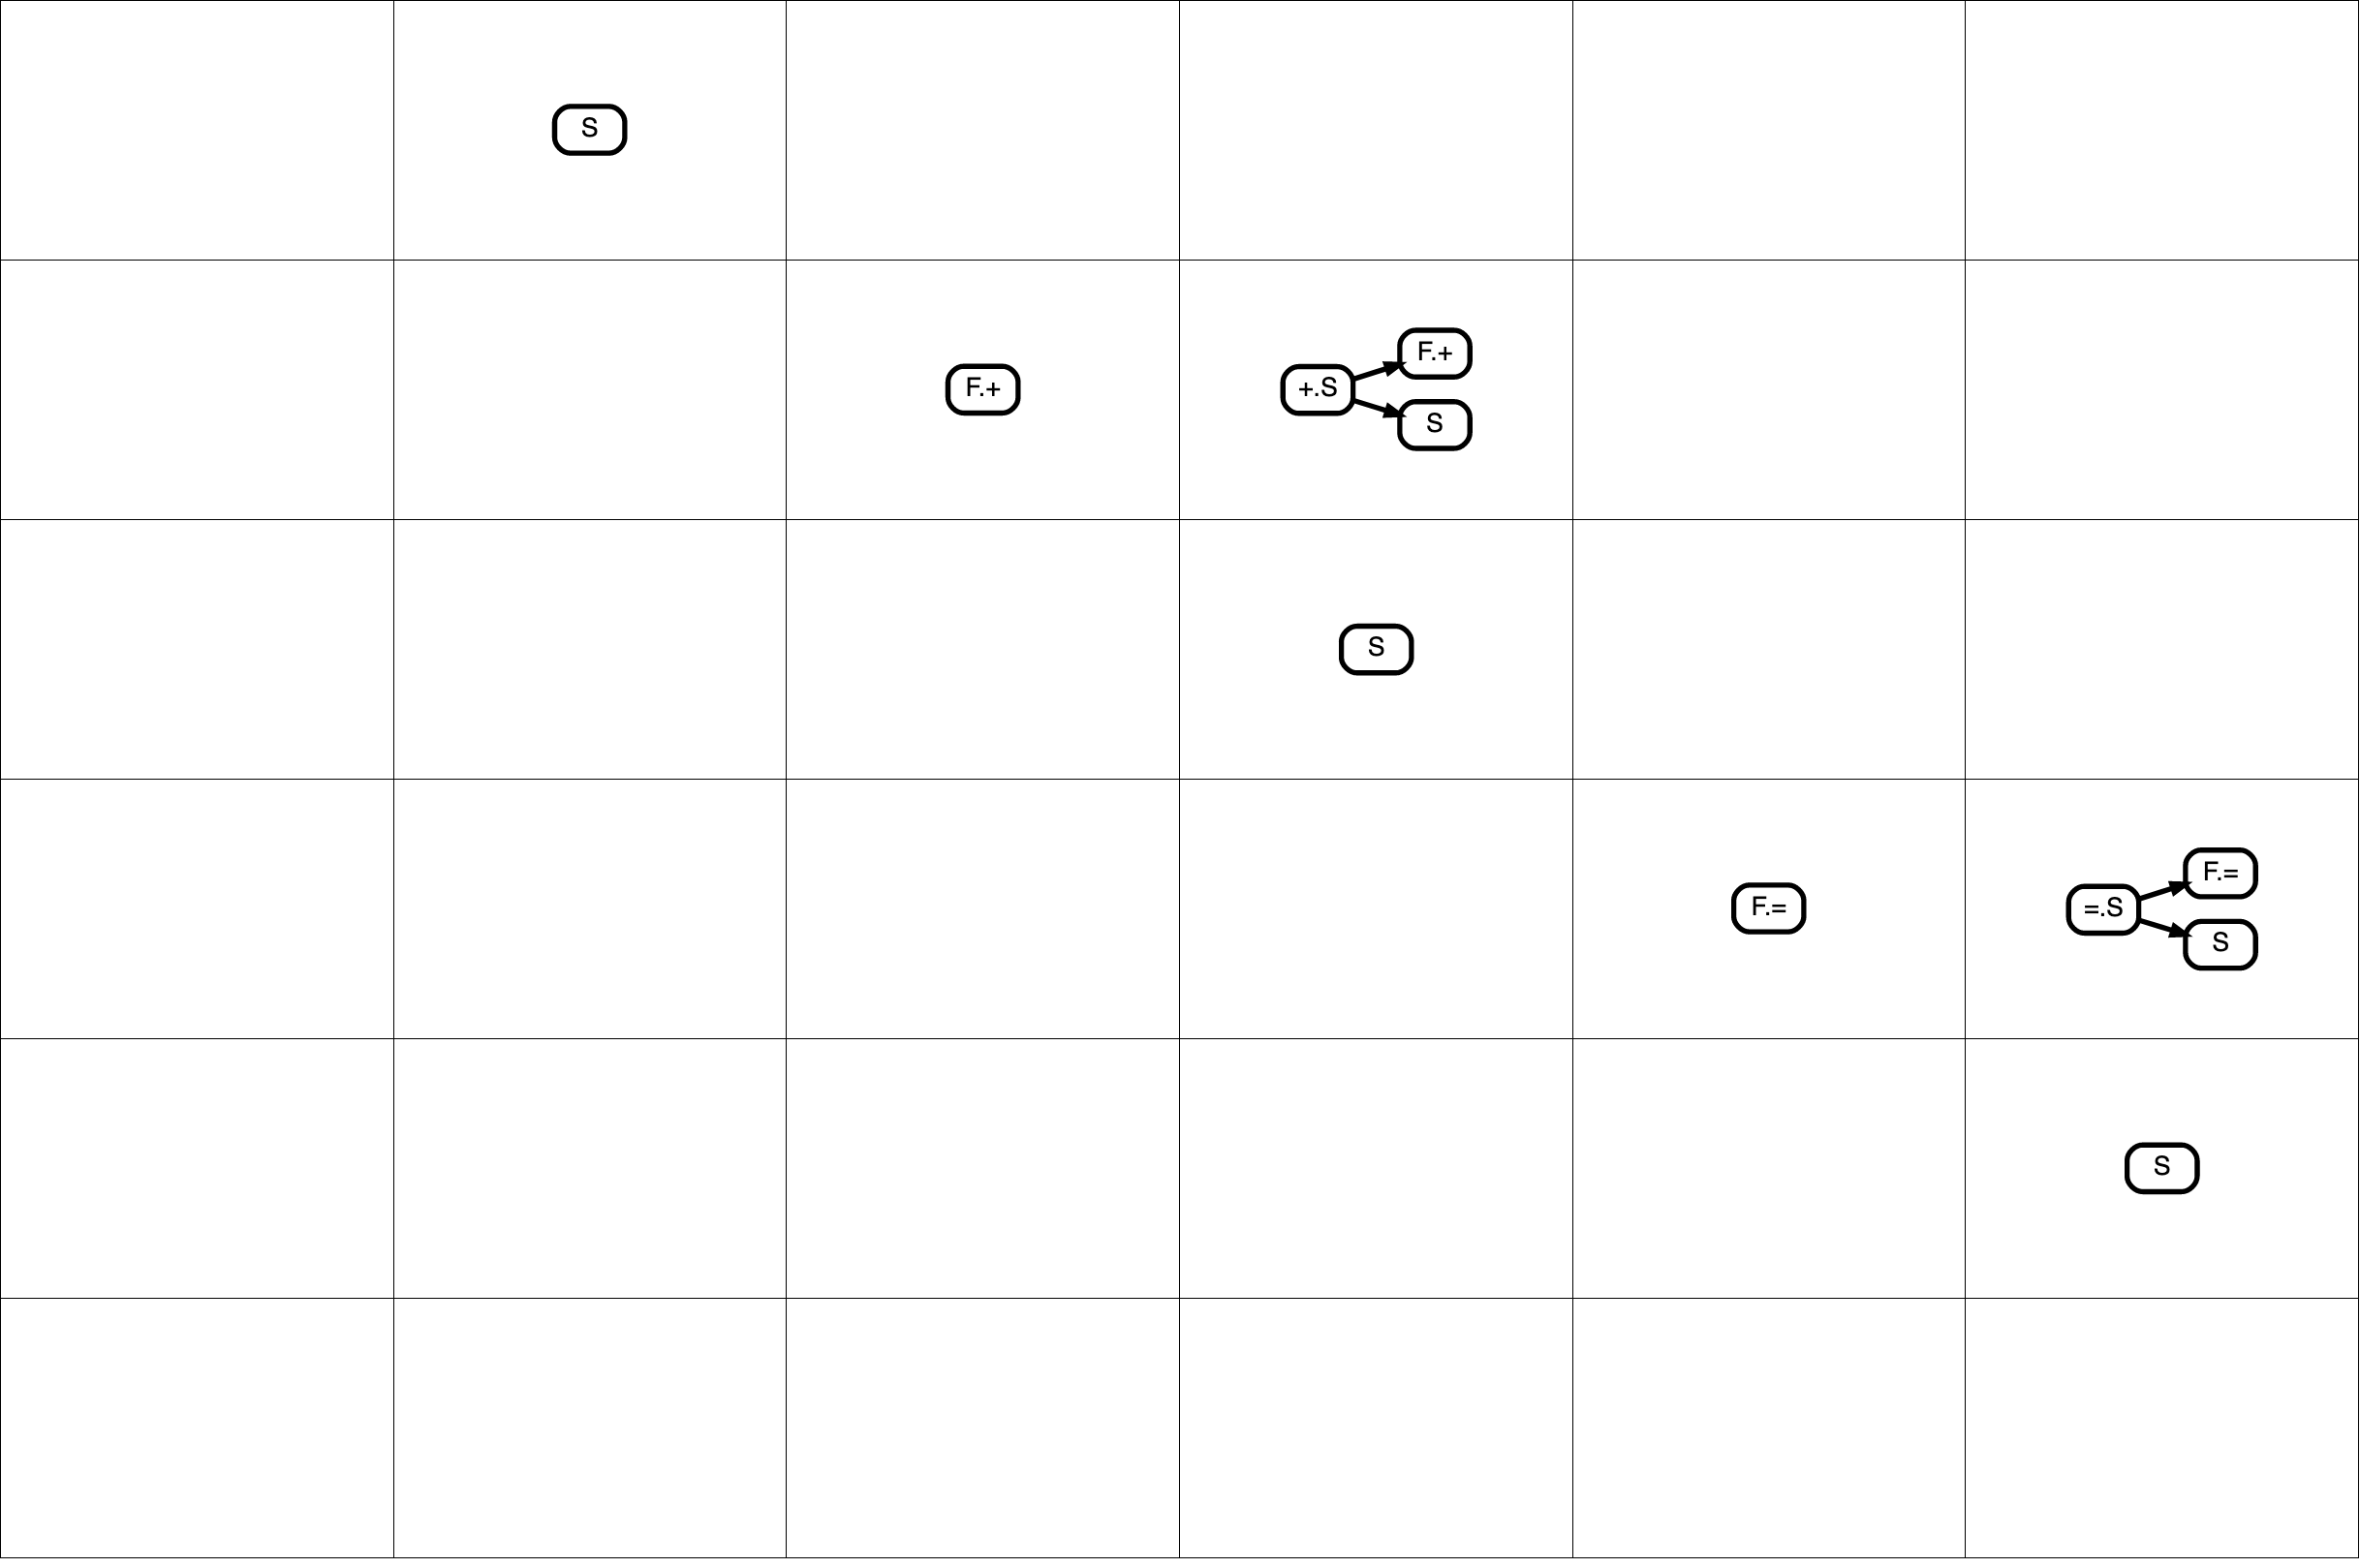
\includegraphics[trim=420 288 0 0,clip, width=12.24cm]{../figures/parse2.png} &
%        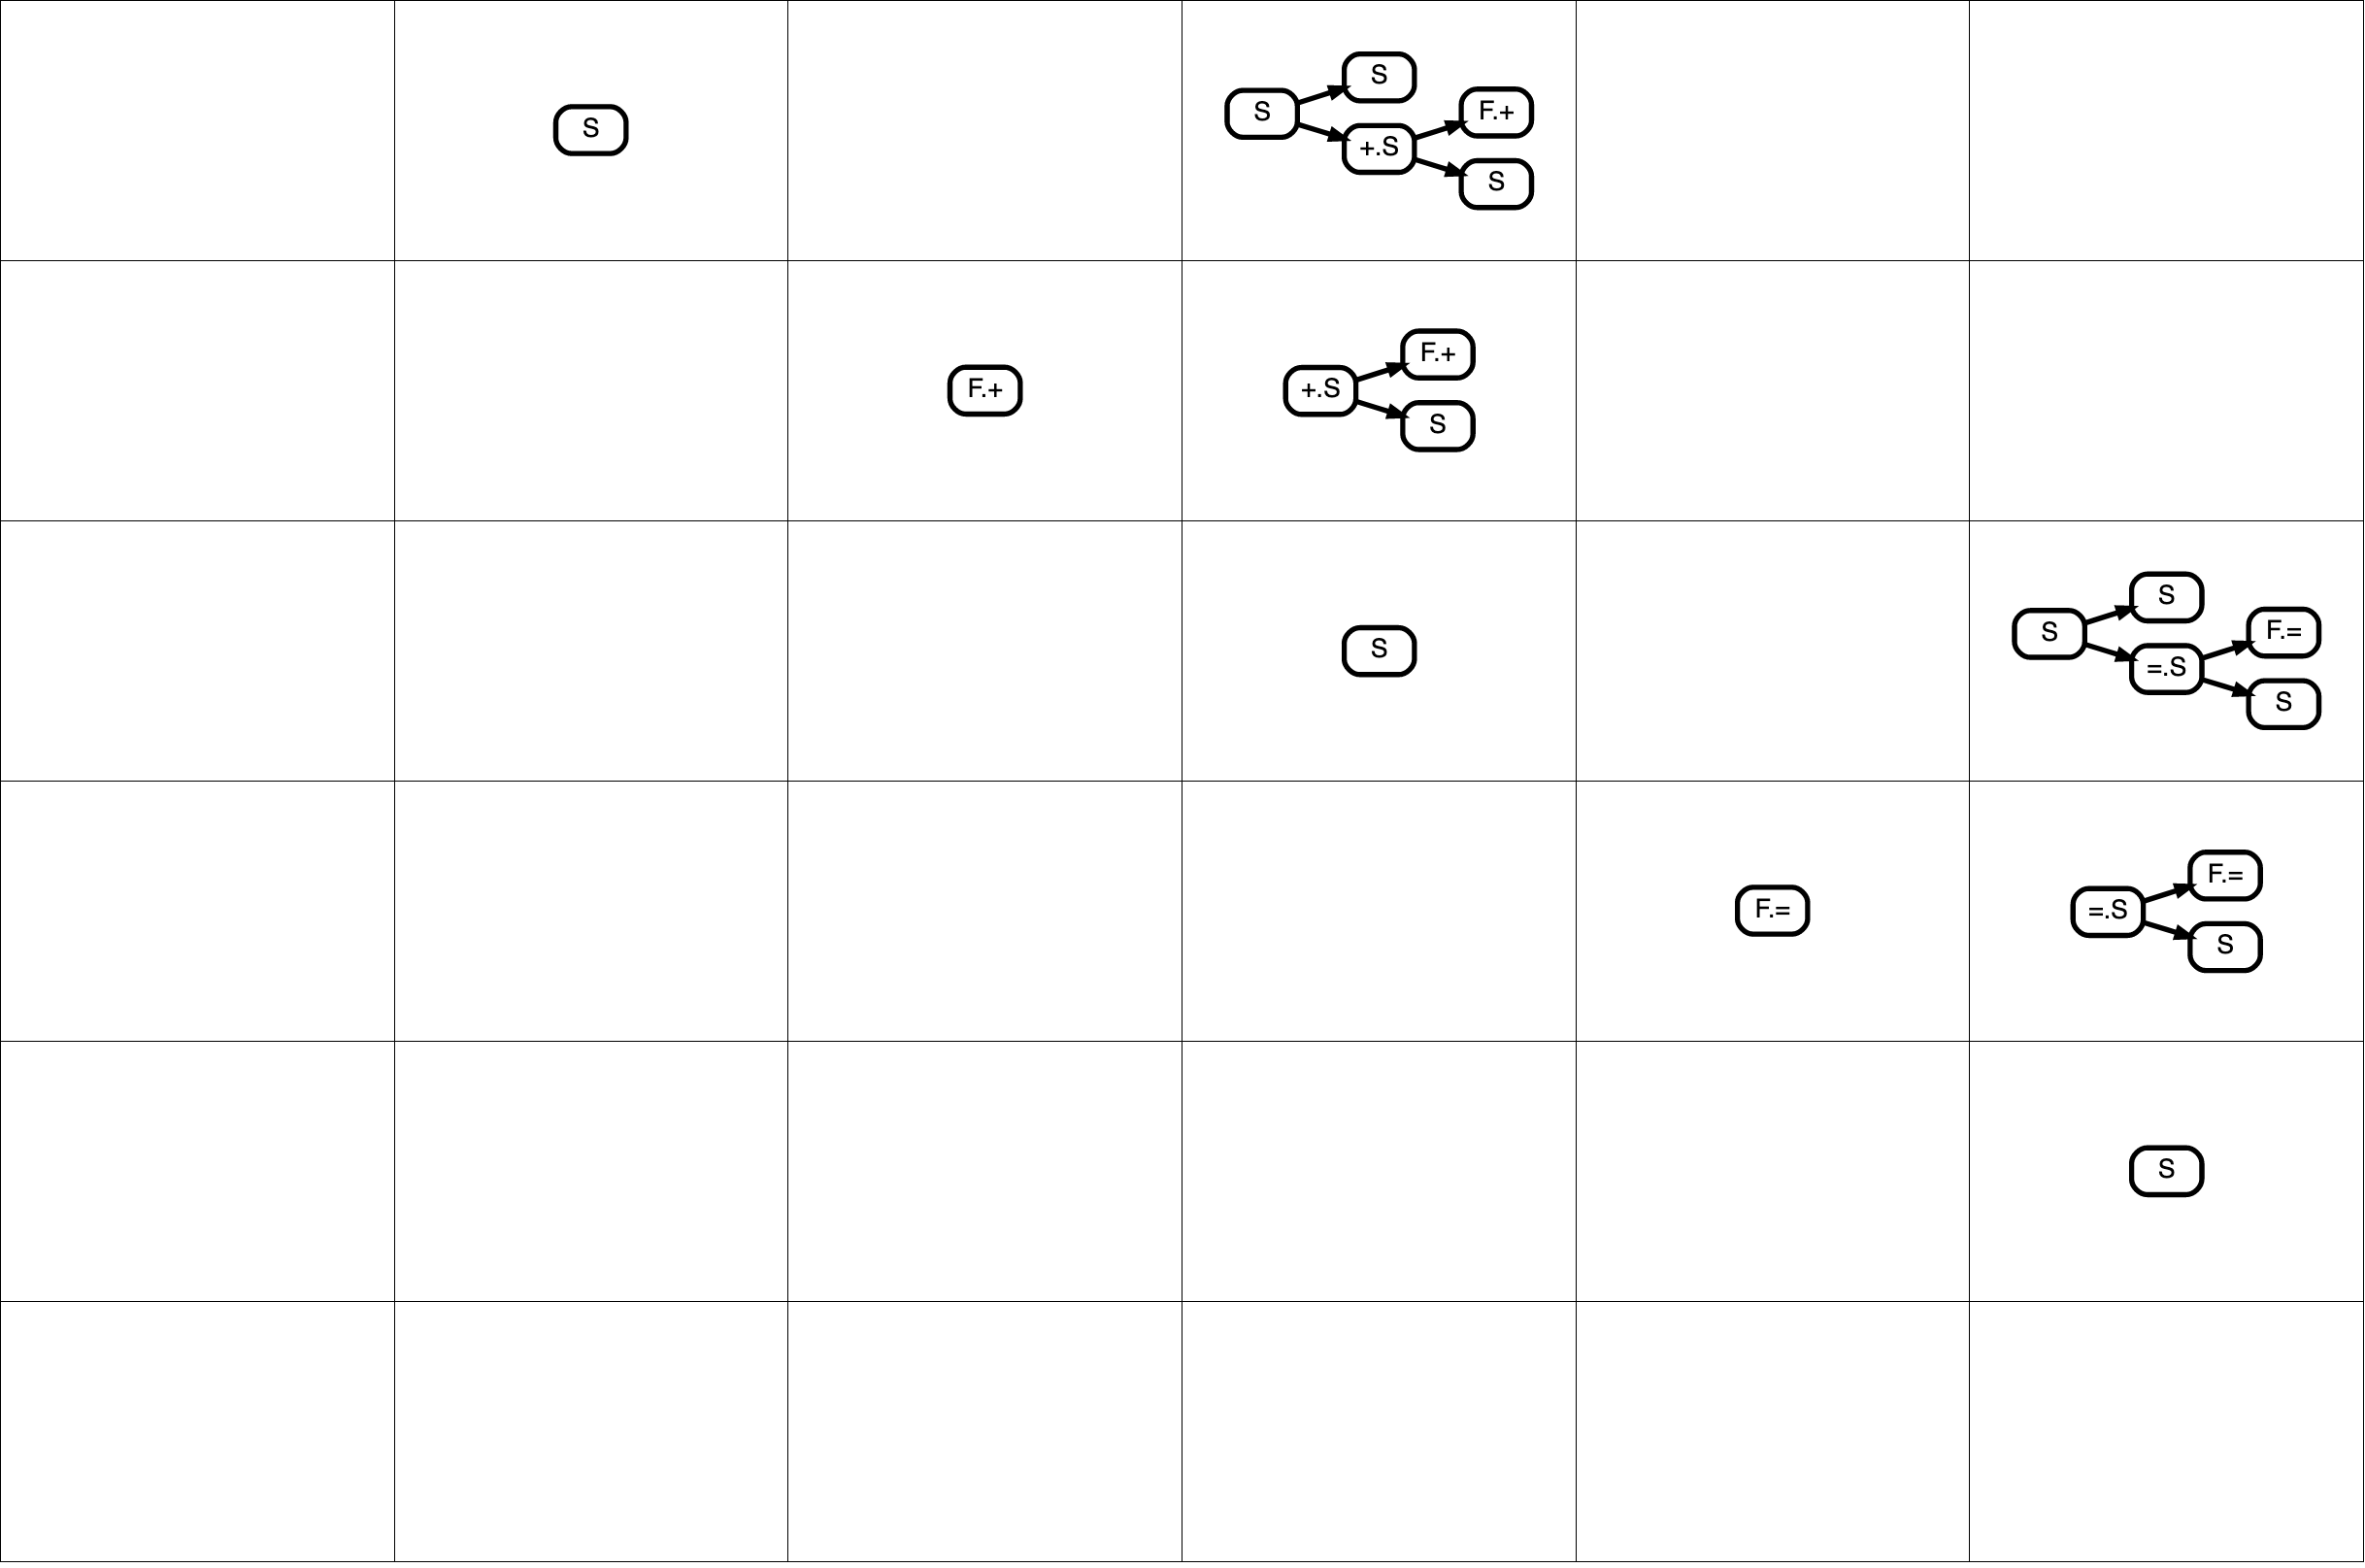
\includegraphics[trim=420 285 0 0,clip, width=12.24cm]{../figures/parse3.png} &
%        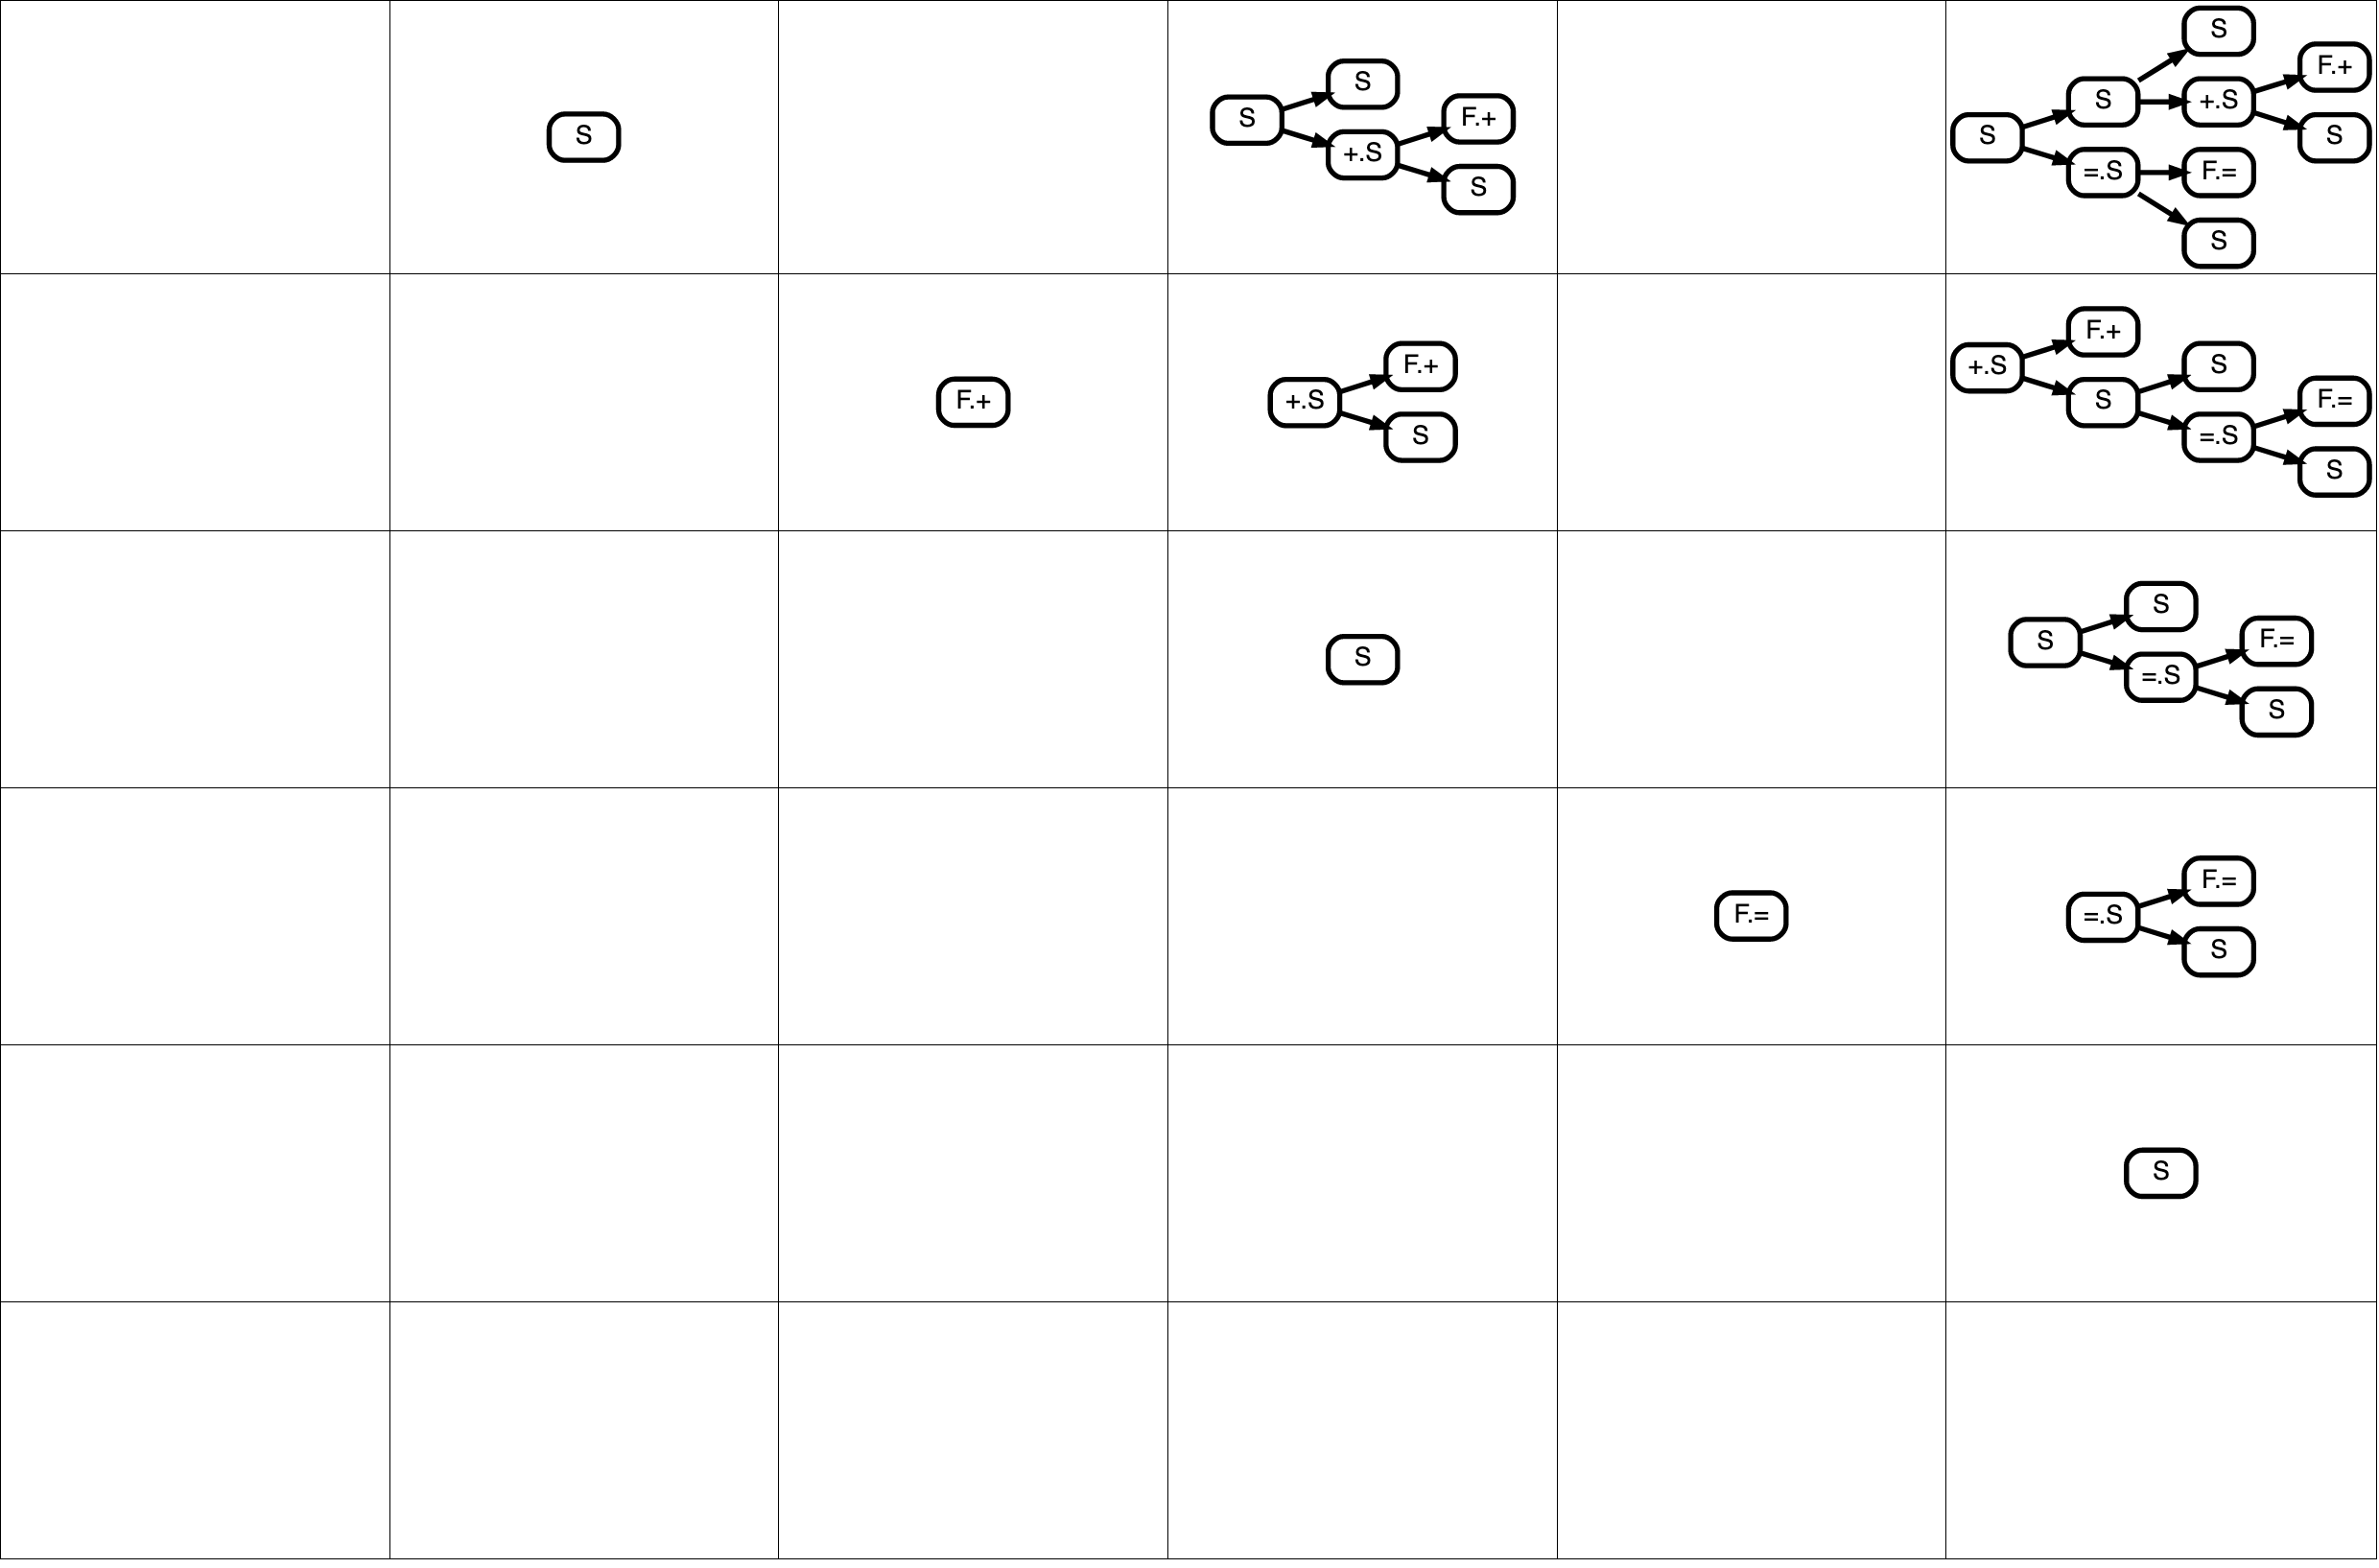
\includegraphics[trim=420 287 0 0,clip, width=12.34cm]{../figures/parse4.png}
%      \end{tabular}
%      \begin{itemize}
%        \item If we had a way to solve for $\mathbf{M = M + M}^2$ directly, power iteration would be unnecessary and we could solve for $\mathbf{M = M}^2$ above the superdiagonal\ldots
%      \end{itemize}
%      \end{minipage}
%      \jointspacing

      \mysection{Galois Connection}
      {\huge
      \null\hspace*{3cm}\begin{minipage}[c]{0.90\columnwidth}
      \begin{itemize}
        \item CYK parser can be lowered onto a tensor $\mathbb{Z}_2^{n\times n \times |V|}$ and $GF(2^{|V|})^{n\times n}$
        \item Binarized CYK parser can be compiled to SAT to solve for $\mathbf{M}^*$ directly
        \item Enables sketch-based synthesis in $\sigma$ or $\mathcal G$: just use variables for holes!
        \item We simply encode the characteristic function, i.e. $\mathds{1}_{\subseteq V}: V\rightarrow \mathbb{B}^{|V|}$
        \item $\oplus, \otimes$ are defined as $\boxplus, \boxtimes$, so that the following diagram commutes:
      \end{itemize}
      \vspace{2cm}
        \adjustbox{scale=0.62,center}{%
          \[\begin{tikzcd}[row sep=large]
            \langle\mathcal{G}', \highlight{\Sigma}^{n-1}\rangle \arrow[leftrightarrow, drrr, shorten=-1mm] & & [-135pt] & \vspace{20pt}\textbf{Set} \arrow[d, phantom] & \textbf{Bit} \arrow[d, phantom] & [-90pt] & \langle\mathcal{G}', \Sigma^{n-1}\rangle \arrow[drr, shorten=-2mm] & [-90pt] & \textbf{SAT} \arrow[d, phantom]\\[-30pt]
            \textbf{Rubix}  \arrow[rr, phantom] & & [-135pt] & M \times M \arrow[r, "\mathds{1}^{2^{n\times n}}", labels=above] \arrow[d, "\hspace{-21mm}\bigoplus\:\bigotimes"] & \mathbb{Z}_2^{|V|^{n\times n}} \times \mathbb{Z}_2^{|V|^{n\times n}} \arrow[d, "\hspace{-23.3mm}\highlight{\mathlarger\boxplus}\:\:\highlight{\mathlarger\boxtimes}"] \arrow[l, "\mathds{1}^{-2^{n\times n}}", labels=below] \arrow[rrrr, rightarrowtail, "\varphi^{2^{n\times n}}", labels=above] & [-90pt] & & [-90pt] & \mathcal{M} \times \mathcal{M} \arrow[llll, rightharpoonup, shorten=3.5mm, "\varphi^{-2^{n\times n}}", labels=below] \arrow[d, "\hspace{-18.5mm}+\:\:\:*"] \\
            \textbf{Matrix} \arrow[rr, phantom] & & [-135pt] & 2^V \times 2^V \arrow[r, "\mathds{1}^{2}", labels=above] \arrow[d, "\hspace{-15.5mm}\oplus\:\otimes"] & \mathbb{Z}_2^{|V|} \times \mathbb{Z}_2^{|V|} \arrow[d, "\hspace{-17.5mm}\highlight{\boxplus}\:\highlight{\boxtimes}"] \arrow[l, "\mathds{1}^{-2}", labels=below] \arrow[rrrr, rightarrowtail, "\varphi^2", labels=above] & [-90pt] & & [-90pt] & \mathcal{V} \times \mathcal{V} \arrow[llll, rightharpoonup, shorten=3.5mm, "\varphi^{-2}", labels=below] \arrow[d, "\hspace{-15.5mm}\boxplus\:\boxtimes"] \arrow[u] \\
            \textbf{Vector} \arrow[rr, phantom] & & [-135pt] & 2^V \arrow[r, "\mathds{1}", labels=above] & \mathbb{Z}_2^{|V|} \arrow[l, "\mathds{1}^{-1}", labels=below] \arrow[rrrr, rightarrowtail, "\varphi", labels=above] & [-90pt] & & [-90pt] & \mathcal{V} \arrow[llll, rightharpoonup, shorten=3.5mm, "\varphi^{-1}", labels=below] \arrow[u]
        \end{tikzcd}\]
        }
%        \item These operators can be lifted into matrices and tensors in the usual way
%        \item In most cases, only a few nonterminals will be active at any given time
%        \item More sophisticated representations are known for $\binom{n}{0 \leq k}$ subsets
%        \item If density is desired, possible to use the Maculay representation
%        \item If you know of a more efficient encoding, please let us know!
      \end{minipage}
      \vspace{6cm}
      }
      \pagebreak

      \jointspacing

      \mysection{Probabilistic Programming}

      {\huge
      \hspace*{3cm}\begin{minipage}[c]{0.90\columnwidth}
      \vspace{1cm}Let $\textbf{R}: \text{GF}(2^{n\times n})$ be a matrix $\mathbf{M}_{0, c} = P_c + \mathbf{M}_{r+1=c} = \top$, where $P$ is a feedback polynomial with coefficients $P_{1\ldots n}$ and $\oplus := \veebar, \otimes := \land$:\\
      \end{minipage}

      \[
        \mathbf{M}^tV = \begin{pNiceMatrix}
          P_1    & \Cdots &        &       & P_n \\
          \top   & \circ  & \Cdots &       & \circ \\
          \circ  & \Ddots & \Ddots &       & \Vdots \\
          \Vdots & \Ddots &        &       &       \\
          \circ  & \Cdots & \circ  & \top  & \circ
        \end{pNiceMatrix}^t
        \begin{pNiceMatrix}
          V_1 \\
          \Vdots \\
              \\
              \\
          V_n
        \end{pNiceMatrix}
      \]\\

      \hspace*{2cm}\begin{minipage}[c]{0.90\columnwidth}
      Selecting any $V \neq \mathbf{0}$ and coefficients $P_j$ from a \textit{primitive polynomial}, then powering the matrix $\mathbf{M}$ generates an ergodic sequence over GF$(2^n)$:\\
      \end{minipage}

      \[
        \mathbf{S} = \begin{pmatrix}V & \mathbf{M}V & \mathbf{M}^{2}V & \mathbf{M}^{3}V & \cdots & \mathbf{M}^{2^n-1}V \end{pmatrix}
      \]

      \vspace{2cm}\hspace*{2cm}\begin{minipage}[c]{0.90\columnwidth}
      This sequence has \textit{full periodicity}, i.e., $\forall i, j \in [0, 2^n), \mathbf{S}_i = \mathbf{S}_j \Rightarrow i = j$.
      \end{minipage}
      }
      \jointspacing

      \mysection{Brozozowski's Derivative}

      \begin{table}
          \begin{tabular}{ccc}
            Left Quotient && Right Quotient \vspace{3pt}\\
            $\frac{\partial f}{\partial \cev{x}} = \big\{\;y \mid (w \rightarrow x y) \in P\;\big\}$ &&
            $\frac{\partial f}{\partial \vec{y}} = \big\{\;x \mid (w \rightarrow x y) \in P\;\big\}$ \vspace{5pt}\\
            \begin{tabular}{|c|c|}
              \hline
              \cellcolor{black!15}x & \cellcolor{black!15}w \\ \hline
              \multicolumn{1}{c|}{~} & y \\
              \cline{2-2}
            \end{tabular} &&
            \begin{tabular}{|c|c|}
              \hline
              x & \cellcolor{black!15}w \\ \hline
              \multicolumn{1}{c|}{~} & \cellcolor{black!15}y \\
              \cline{2-2}
            \end{tabular}
          \end{tabular}
      \end{table}

      \definecolor{R}{RGB}{202,65,55}
      \definecolor{G}{RGB}{151,216,56}
      \definecolor{W}{RGB}{255,255,255}
      \definecolor{X}{RGB}{65,65,65}

      \newcommand{\TikZRubikFaceLeft}[9]{\def\myarrayL{#1,#2,#3,#4,#5,#6,#7,#8,#9}}
      \newcommand{\TikZRubikFaceRight}[9]{\def\myarrayR{#1,#2,#3,#4,#5,#6,#7,#8,#9}}
      \newcommand{\TikZRubikFaceTop}[9]{\def\myarrayT{#1,#2,#3,#4,#5,#6,#7,#8,#9}}
      \newcommand{\BuildArray}{\foreach \X [count=\Y] in \myarrayL%
      {\ifnum\Y=1%
      \xdef\myarray{"\X"}%
      \else%
      \xdef\myarray{\myarray,"\X"}%
      \fi}%
      \foreach \X in \myarrayR%
      {\xdef\myarray{\myarray,"\X"}}%
      \foreach \X in \myarrayT%
      {\xdef\myarray{\myarray,"\X"}}%
      \xdef\myarray{{\myarray}}%
      }
      \TikZRubikFaceLeft
      {LA}{W}{W}
      {W}{LB}{LC}
      {LD}{W}{W}
      \TikZRubikFaceRight
      {W}{LK}{W}
      {LC}{W}{LG}
      {W}{LH}{W}
      \TikZRubikFaceTop
      {LA}{W}{LI}
      {W}{W}{LJ}
      {W}{LK}{W}
      \BuildArray
      \pgfmathsetmacro\radius{0.1}
      \tdplotsetmaincoords{55}{135}

      \showcellnumberfalse

      \bgroup
      \newcommand\ddd{\Ddots}
      \newcommand\vdd{\Vdots}
      \newcommand\cdd{\Cdots}
      \newcommand\lds{\ldots}
      \newcommand\vno{\varnothing}
      \newcommand{\ts}[1]{\textsuperscript{#1}}
      \newcommand\non{1\ts{st}}
      \newcommand\ntw{2\ts{nd}}
      \newcommand\nth{3\ts{rd}}
      \newcommand\nfo{4\ts{th}}
      \newcommand\nfi{5\ts{th}}
      \newcommand\nsi{6\ts{th}}
      \newcommand\nse{7\ts{th}}
      \newcommand\rcr{\rowcolor{black!15}}
      \newcommand\rcw{\rowcolor{white}}
      \newcommand\pcd{\cdot}
      \newcommand\pcp{\phantom\cdot}
      \newcommand\ppp{\phantom{\nse}}

        \[
          \begin{align*}
            o &\rightarrow \hiliD{so} \mid \hiliC{rs} \mid \hiliB{rr}\hspace{0.5pt} \mid \hiliA{oo}\\
            r &\rightarrow \hiliE{so} \mid \hiliH{ss}\hspace{0.4pt}\mid \hiliF{rr}\hspace{0.5pt} \mid \hiliK{os}\\
            s &\rightarrow \hiliL{so} \mid \hiliG{rs} \mid \hiliJ{or} \mid \hiliI{oo}
          \end{align*} \phantom{=} \mathcal{H}_{\{o\}} = \begin{pmatrix}
                 \hiliA{\pder{^2 o}{\cev{o}\partial\vec{o}}} & \pder{^2 o}{\cev{o}\partial\vec{r}} & \pder{^2 o}{\cev{o}\partial\vec{s}}\\
                 \pder{^2 o}{\cev{r}\partial\vec{o}} & \hiliB{\pder{^2 o}{\cev{r}\partial\vec{r}}} & \hiliC{\pder{^2 o}{\cev{r}\partial\vec{s}}}\\
                 \hiliD{\pder{^2 o}{\cev{s}\partial\vec{o}}} & \pder{^2 o}{\cev{s}\partial\vec{r}} & \pder{^2 o}{\cev{s}\partial\vec{s}}
          \end{pmatrix}
%    \mathcal{J} = \begin{pmatrix}
%       \pder{o}{o} & \pder{o}{r} & \pder{o}{s}\\
%       \pder{r}{o} & \pder{r}{r} & \pder{r}{s}\\
%       \pder{s}{o} & \pder{s}{r} & \pder{s}{s}
%    \end{pmatrix}
        \]
        \hspace{-0.5cm}\begin{minipage}[l]{25cm}
         \scalebox{2}{\begin{tikzpicture}
                \clip (-3,-2.5) rectangle (3,2.5);
                \begin{scope}[tdplot_main_coords]
                  \filldraw [canvas is yz plane at x=1.5] (-1.5,-1.5) rectangle (1.5,1.5);
                  \filldraw [canvas is xz plane at y=1.5] (-1.5,-1.5) rectangle (1.5,1.5);
                  \filldraw [canvas is yx plane at z=1.5] (-1.5,-1.5) rectangle (1.5,1.5);
                  \foreach \X [count=\XX starting from 0] in {-1.5,-0.5,0.5}{
                    \foreach \Y [count=\YY starting from 0] in {-1.5,-0.5,0.5}{
                      \pgfmathtruncatemacro{\Z}{\XX+3*(2-\YY)}
                      \pgfmathsetmacro{\mycolor}{\myarray[\Z]}
                      \draw [thick,canvas is yz plane at x=1.5,shift={(\X,\Y)},fill=\mycolor] (0.5,0) -- ({1-\radius},0) arc (-90:0:\radius) -- (1,{1-\radius}) arc (0:90:\radius) -- (\radius,1) arc (90:180:\radius) -- (0,\radius) arc (180:270:\radius) -- cycle;
                      \ifshowcellnumber
                      \node[canvas is yz plane at x=1.5,shift={(\X+0.5,\Y+0.5)}] {\Z};
                      \fi
                      \pgfmathtruncatemacro{\Z}{2-\XX+3*(2-\YY)+9}
                      \pgfmathsetmacro{\mycolor}{\myarray[\Z]}
                      \draw [thick,canvas is xz plane at y=1.5,shift={(\X,\Y)},fill=\mycolor] (0.5,0) -- ({1-\radius},0) arc (-90:0:\radius) -- (1,{1-\radius}) arc (0:90:\radius) -- (\radius,1) arc (90:180:\radius) -- (0,\radius) arc (180:270:\radius) -- cycle;
                      \ifshowcellnumber
                      \node[canvas is xz plane at y=1.5,shift={(\X+0.5,\Y+0.5)},xscale=-1] {\Z};
                      \fi
                      \pgfmathtruncatemacro{\Z}{2-\YY+3*\XX+18}
                      \pgfmathsetmacro{\mycolor}{\myarray[\Z]}
                      \draw [thick,canvas is yx plane at z=1.5,shift={(\X,\Y)},fill=\mycolor] (0.5,0) -- ({1-\radius},0) arc (-90:0:\radius) -- (1,{1-\radius}) arc (0:90:\radius) -- (\radius,1) arc (90:180:\radius) -- (0,\radius) arc (180:270:\radius) -- cycle;
                      \ifshowcellnumber
                      \node[canvas is yx plane at z=1.5,shift={(\X+0.5,\Y+0.5)},xscale=-1,rotate=-90] {\Z};
                      \fi
                    }
                  }
                  \draw [decorate,decoration={calligraphic brace,amplitude=10pt,mirror},yshift=0pt, line width=1.25pt]
                  (3,0) -- (3,3) node [black,midway,xshift=-8pt, yshift=-14pt] {\footnotesize $V_x$};
                  \draw [decorate,decoration={calligraphic brace,amplitude=10pt},yshift=0pt, line width=1.25pt]
                  (3,0) -- (0,-3) node [black,midway,xshift=-16pt, yshift=0pt] {\footnotesize $V_y$};
                  \draw [decorate,decoration={calligraphic brace,amplitude=10pt},yshift=0pt, line width=1.25pt]
                  (0,-3) -- (-3,-3) node [black,midway,xshift=-8pt, yshift=14pt] {\footnotesize $V_w$};
                \end{scope}
         \end{tikzpicture}}
        \end{minipage}
        \begin{minipage}[c]{25.5cm}
          \begin{align*}
            \mathcal{H}_{\{r\}} = & \begin{pmatrix}
                      \pder{^2 r}{\cev{o}\partial\vec{o}} & \pder{^2 r}{\cev{o}\partial\vec{r}} & \hiliK{\pder{^2 r}{\cev{o}\partial\vec{s}}}\\
                      \pder{^2 r}{\cev{r}\partial\vec{o}} & \hiliF{\pder{^2 r}{\cev{r}\partial\vec{r}}} & \pder{^2 r}{\cev{r}\partial\vec{s}}\\
                      \hiliE{\pder{^2 r}{\cev{s}\partial\vec{o}}} & \pder{^2 r}{\cev{s}\partial\vec{r}} & \hiliH{\pder{^2 r}{\cev{s}\partial\vec{s}}}
            \end{pmatrix}
          \end{align*}
          \begin{align*}
            \mathcal{H}_{\{s\}} = & \begin{pmatrix}
                      \hiliI{\pder{^2 s}{\cev{o}\partial\vec{o}}} & \hiliJ{\pder{^2 s}{\cev{o}\partial\vec{r}}} & \pder{^2 s}{\cev{o}\partial\vec{s}}\\
                      \pder{^2 s}{\cev{r}\partial\vec{o}} & \pder{^2 s}{\cev{r}\partial\vec{r}} & \hiliG{\pder{^2 s}{\cev{r}\partial\vec{s}}}\\
                      \hiliL{\pder{^2 s}{\cev{s}\partial\vec{o}}} & \pder{^2 s}{\cev{s}\partial\vec{r}} & \pder{^2 s}{\cev{s}\partial\vec{s}}
            \end{pmatrix}
          \end{align*}
        \end{minipage}

      {\huge
      \hspace*{3cm}\begin{minipage}[c]{0.90\columnwidth}
       \vspace{1cm}It is well-known that the family of CFLs is not closed under intersection. For example, consider $\mathcal{L}_\cap := \mathcal{L}(\mathcal{G}_1) \cap \mathcal{L}(\mathcal{G}_1)$:

      \begin{table}[H]
        \begin{tabular}{llll}
          $P_1 := \big\{\;S \rightarrow L R,$ & $L \rightarrow a b \mid a L b,$ & $R \rightarrow c \mid c R\;\big\}$\vspace{5pt}\\
          $P_2 := \big\{\;S \rightarrow L R,$ & $R \rightarrow b c \mid b R c,$ & $L \rightarrow a \mid a L\;\big\}$
        \end{tabular}
      \end{table}

         $\mathcal{L}_\cap$ generates the language $\big\{\;a^d b^d c^d \mid d > 0\;\big\}$, which is not context free.
      \end{minipage}
      }

    \end{multicols}


    \bottombox{
    %% QR code
    %    \hfill\bottomboxlogo{img/kotlin_logo.png}
    % Comment out the line below out to hide logo
    \hspace{4cm}
    \begin{minipage}[c][0.1\paperheight][c]{0.18\textwidth}\qrcode[height=2.6in]{ssnp.ndan.co} \end{minipage}
    \begin{minipage}[c][0.1\paperheight][c]{0.25\textwidth}
\includegraphics[height=2.6in]{../figures/fpt_logo.png} \end{minipage}
    \begin{minipage}[c][0.1\paperheight][c]{0.33\textwidth}
\includegraphics[height=2.6in]{../figures/mcgill.png} \end{minipage}
    \begin{minipage}[c][0.1\paperheight][c]{0.33\textwidth}
\includegraphics[height=3.2in]{../figures/mila.png} \end{minipage}
    %    \hfill\bottomboxlogo{img/mila_mauve.png} % \hfill shifts the logo across so it meets the right hand side margin
    % Note that \bottomboxlogo takes an optional width argument. It defaults to the following:
    % \hfill\bottomboxlogo[width=\textwidth]{<path_to_image_file>}
    % where \textwidth is actually the width of a minipage which is defined in the \bottombox command of
    % betterportaitposter.cls It's a standard \includegraphics command in there, so easy to change if
    % you need to add a border etc.
    }
\end{poster}
\end{document}
